\section{Anleitungen}
\label{sec:anleitungen}
Diese Anleitungen sind an dem zukünftigen Entwickler dieser Prototyp gerichtet. Mithilfe dieser Dokumentation und des mitgelieferten Images der Aussensprechstelle, soll ein Entwickler im Stand sein eine neu installierte Raspbian \gls{os} einer Aussensprechstelle/Server zu konfigurieren. Alles was konfiguriert wurde, wurde dokumentiert und in der Anleitung aufgeführt. Diese soll auch das Hinzufügen zukünftiger Funktionalitäten erleichtern.

\subsection{Aussensprechstelle Konfigurationsanleitung}

\subsubsection{Aktuelle Stand}
Betriebssystem:	Raspbian jessie with pixel\\
Version: April 2017\\
Kernel Version: 4.4

\subsubsection{Namen und Passwortkonzept}
Hostname: DoorPixxx (x= fortlaufende Nummerierung)\\
User: pi\\
Password: bachelor (Einfachheitshalber wurde dieses schwache Passwort ausgewählt. Sollte aber bei einer produktiven Inbetriebnahme zwingend geändert werden)\\

\subsubsection{Betriebssystem Installation}
\begin{itemize}
	\item Das Image von raspberry.com herunterladen und extrahieren \\ (https://www.raspberrypi.org/downloads/raspbian/)
	\item Um die Image auf der SD Karte zu bringen benutzt man Etcher.  (https://etcher.io/)
	\item Mit den Standard-Anmeldedaten Anmelden. User: pi Password: raspberry
\end{itemize}



\subsubsection{Allgemeine Einstellungen}
Das System soll auf dem neusten Stand aktualisieren werden
\begin{lstlisting}[backgroundcolor = \color{snippetcolor},
language = bash,
xleftmargin = 1cm,
framexleftmargin = 0.1em,
breaklines=true]
	apt-get update 
	sudo apt-get upgrade
\end{lstlisting}

Mit dem Terminalkommando ’sudo raspi-config’ können durch eine grafische Oberfläche folgende allgemeine Einstellungen angepasst werden:
\begin{itemize}
	\item Unter 'Interfacing Options' muss die SSH Server aktiviert werden.
	\item Hostname gemäss Namenskonzept anpassen
	\item Neue Passwort für den Pi Benutzer gemäss Password Konzept setzen.
	\item Zum Schluss sollen auch die Zeitzone, das Land und das Tastaturlayout angepasst werden.
\end{itemize}

\subsubsection{Bidschirm Konfiguration}
Die Displaytreiber von waveshare.com herunterladen und auf die SD Karte in Root Directory speichern. (http://www.waveshare.com/wiki/4inch\char`_HDMI\char`_LCD)\\
Mit folgenden Bash-Kommandos wird der Treiber installiert:
\begin{lstlisting}[backgroundcolor = \color{snippetcolor},
language = bash,
xleftmargin = 1cm,
framexleftmargin = 0.1em,
breaklines=true]
	tar xzvf /boot/LCD-show-YYMMDD.tar.gz 
	cd LCD-show/
	chmod +x LCD4-800x480-show
	./LCD4-800x480-show
\end{lstlisting}
Nachdem dass der Bildschirmtreiber installiert wurde, müssen die Einstellungen für den Bildschirm angepasst werden. Folgende Code-Zeilen müssen am Ende der ’config.txt’ Datei, die sich in der root-directory befindet, hinzugefügt werden \cite{displayConfig}.
\begin{lstlisting}[backgroundcolor = \color{snippetcolor},
language = bash,
xleftmargin = 1cm,
framexleftmargin = 0.1em,
breaklines=true]
	hdmi_group=2
	hdmi_mode=87
	hdmi_cvt 480 800 60 6 0 0 0
	dtoverlay=ads7846,cs=1,penirq=25,penirq_pull=2,
	speed=50000,keep_vref_on=0,swapxy=0,pmax=255,
	xohms=150,xmin=200,xmax=3900,ymin=200,ymax=3900
	display_rotate=3
\end{lstlisting}

\subsubsection{Browser Kiosk-mode}
Als erstes wird das Unclutter-Tool installiert um den Mausepfeil auszublenden.
\begin{lstlisting}[backgroundcolor = \color{snippetcolor},
language = bash,
xleftmargin = 1cm,
framexleftmargin = 0.1em,
breaklines=true]
	sudo apt-get install unclutter
\end{lstlisting}
Die Kiosk-Mode-Einstellungen werden in der config Datei  \\ (/home/pi/.config/lxsession/LXDE-pi/autostart) wie folgt angepasst
\begin{lstlisting}[backgroundcolor = \color{snippetcolor},
language = bash,
xleftmargin = 1cm,
framexleftmargin = 0.1em,
breaklines=true]
	# Chromium auto start in kiosk mode
	# path: /home/pi/.config/lxsession/LXDE-pi/autostart
	@lxpanel --profile LXDE-pi
	@pcmanfm --desktop --profile LXDE-pi
	#@xscreensaver -no-splash
	@point-rpi
	@xset s off
	@xset s noblank
	@xset -dpms
	@chromium-browser --noerrdialogs --kiosk --incognito https://172.16.111.99/server
\end{lstlisting}

\subsubsection{Aussensprechstelle Initialisierung}
Im Homeverzeichnis unter .config/autostart wird die Datei Aussensprechstelle.desktop erstellt.
\begin{lstlisting}[backgroundcolor = \color{snippetcolor},
language = bash,
xleftmargin = 1cm,
framexleftmargin = 0.1em,
breaklines=true]
	touch /home/pi/Aussensprechstelle/Startup/AussensprechstelleLauncher.sh
\end{lstlisting}
Inhalt des Scripst:
\begin{lstlisting}[backgroundcolor = \color{snippetcolor},
language = bash,
xleftmargin = 1cm,
framexleftmargin = 0.1em,
breaklines=true]
	#!/bin/bash
	# This script executes the needed commands on startup to initialize the Aussensprechstelle
	# /home/pi/Aussensprechstelle/Startup/AussensprechstelleLauncher.sh
	#
	# Activates the Camera Driver (Safe mode because of the chrome resolution bug)
	sudo modprobe bcm2835-v4l2 gst_v4l2src_is_broken=1
	#
	# Clears the old TasterController PID of the process (In case of system shutdown)
	file="/var/run/TasterController.pid"
	if [ -f $file ] ; then
		rm $file
	fi
	#
	# Starts the TasterController
	sudo java -jar /home/pi/Aussensprechstelle/TasterController/TasterController.jar &
	#
	# Creates the PID for the taster controller
	sudo echo $! > /var/run/TasterController.pid
	#
	# Starts the watchdog service
	sudo service watchdog start	
\end{lstlisting}

\subsubsection{Taster Controller}
Der Tastencontroller, der für den Key Mapping zuständig ist, wird vom oben gezeigten AussensprechstelleLauncher.sh unter /home/pi/Aussensprechstelle/TasterController/TasterController.jar gestartet. Die kompilierte Jar-Artefakt  muss also dorthin kopiert werden. 
\\
Folgende GPIO Pins werden von den 3 Tasten benötigt um die Aussensprechstelle zu steuern:
\begin{itemize}
	\item GPIO17(16) simuliert den Tastendruck J «Links navigieren»
	\item GPIO27(20) simuliert den Tastendruck K «Anrufen»
	\item GPIO22(21) simuliert den Tastendruck L «Rechts navigieren»
\end{itemize}

\subsubsection{Speaker Controller Service}
Als Erstes muss der mitgelieferte Jar Artefakt SpeakerController.jar unter folgenden Pfad kopiert werden:
\begin{lstlisting}[backgroundcolor = \color{snippetcolor},
language = bash,
xleftmargin = 1cm,
framexleftmargin = 0.1em,
breaklines=true]
	/home/door/Aussensprechstelle/SpeakerController/SpeakerController.jar
\end{lstlisting}
Um den Speaker-Controller als Service unter Unix laufen zu lassen, muss unter /etc/init.d/ das Speaker-Controller-Script erzeugt werden. Der Inhalt des Scripts wird mit dem Projekt mitgeliefert. Um es ausführbar zu machen, muss noch die
«execute» Berechtigung gegeben werden.

\begin{lstlisting}[backgroundcolor = \color{snippetcolor},
language = bash,
xleftmargin = 1cm,
framexleftmargin = 0.1em,
breaklines=true]
	touch /etc/init.d/speakerController
	chmod +x /etc/init.d/speakerController
\end{lstlisting}
Damit der SpeakerController-Service auch automatisch beim Systemstart ausgeführt wird, muss noch folgendes Kommando ausgeführt werden:
\begin{lstlisting}[backgroundcolor = \color{snippetcolor},
language = bash,
xleftmargin = 1cm,
framexleftmargin = 0.1em,
breaklines=true]
	sudo update-rc.d speakerController defaults
\end{lstlisting}
Der Speaker Controller kann nun mit folgenden Befehlen gestartet und gestoppt werden
\begin{lstlisting}[backgroundcolor = \color{snippetcolor},
language = bash,
xleftmargin = 1cm,
framexleftmargin = 0.1em,
breaklines=true]
	sudo service speakerController start
	sudo service speakerController stop
	sudo service speakerController restart
	sudo service speakerController status
\end{lstlisting}

\subsubsection{Watchdog/Watchdog deamon}
Um die von der Aussensprechstelle benötigte Dienste zu überwachen, wird ein Watchdog verwendet. Raspberry Pi hat ein «stad-alone» Hardware Watchdog die ein Autostart durchführt sobald eine der Dienste oder den OS still steht.
Mit folgenden Kommandos wird der Watchdog installiert:
\\
\begin{lstlisting}[backgroundcolor = \color{snippetcolor},
language = bash,
xleftmargin = 1cm,
framexleftmargin = 0.1em,
breaklines=true]
	sudo modprobe bcm2835-wdt
	sudo apt-get install watchdog chkconfig
	sudo chkconfig watchdog on
	sudo /etc/init.d/watchdog start
\end{lstlisting}
Damit die SpeakerController und die TasterController vom Watchdog überwacht werden, muss unter /etc/watchdog.conf die Konfigurationsdatei abgeändert werden. Der Inhalt der Konfigurationsdatei wird mit dem Projekt mitgeliefert.


\subsection{Server Konfigurationsanleitung}
\subsubsection{Aktuelle Stand}
Betriebssystem:	Raspbian jessie with pixel\\
Version: April 2017\\
Kernel Version: 4.4

\subsubsection{Namen und Passwortkonzept}
Hostname: SrvPixxx (x= fortlaufende Nummerierung)\\
User: pi\\
Password: raspberry (Default Password)\\


\subsubsection{Software Installation}
Nun werden die benötigten Dienste und Tools installiert, die vom Server benötigt werden.

\begin{itemize}
	\item Installation der Webserver. (PHP, Nginx, MySQL, Java SDK, Composer,
	Utils)
\end{itemize}

\begin{lstlisting}[backgroundcolor = \color{snippetcolor},
language = bash,
xleftmargin = 0.5cm,
framexleftmargin = 0.1em,
breaklines=true]
	apt-get install nginx
	udo apt-get install mysql-server
	apt-get install php5-fpm php5-mysql
	sudo apt-get install mysql-server mysql-client
	sudo apt-get install oracle-java8-jdk
	sudo apt-get install curl php5-cli git
	curl -sS https://getcomposer.org/installer | sudo php -- --install-dir=/usr/local/bin --filename=composer
\end{lstlisting}

\subsubsection{Erstellung SSL Zertifikate}
\label{kap:zertifikategen}
Bevor die Webapplikationen installiert werden können, müssen die Zertifikate generiert werden (Self-Signed).

\begin{itemize}
	\item Erstellung SSL Zertifikat für den Client Webapplikation. Als Hostname wird hier als Beispiel intercom.app verwendet. Zuerst muss eine Konfigurationsdatei (v3.ext) mit folgendem Inhalt generiert werden:
\end{itemize}

\begin{lstlisting}[backgroundcolor = \color{snippetcolor},
language = bash,
xleftmargin = 0.5cm,
framexleftmargin = 0.1em,
breaklines=true]
	authorityKeyIdentifier=keyid,issuer
	basicConstraints=CA:TRUE
	keyUsage = digitalSignature, nonRepudiation, keyEncipherment, dataEncipherment
	subjectAltName = @alt_names
	
	[alt_names]
	DNS.1 = intercom.app
\end{lstlisting}
Falls ein IP als hostname verwendet wird, kann man \texttt{@alt\_names} mit IP:192.168.0.18 ersetzen.

\begin{itemize}
	\item 
	Nun müssen folgende Befehle eingegeben werden. Wenn gefragt, muss der Hostname oder IP als Common Name (CN) eingegeben werden. Es kann immer das gleiche Passwort verwendet werden und muss dem Keystore-Password des Signaling-Servers entsprechen.
\end{itemize}

\begin{lstlisting}[backgroundcolor = \color{snippetcolor},
xleftmargin = 0.5cm,
framexleftmargin = 0.1em,
breaklines=true]
	sudo openssl genrsa -des3 -out rootCA.key 2048
	
	sudo openssl req -x509 -new -nodes -key rootCA.key -sha256 -days 1024 -out rootCA.pem
	
	sudo openssl req -new -sha256 -nodes -out server.csr -newkey rsa:2048 -keyout server.key
	
	sudo openssl x509 -req -in server.csr -CA rootCA.pem -CAkey rootCA.key -CAcreateserial -out server.crt -days 500 -sha256 -extfile v3.ext
	
	sudo openssl pkcs12 -export -in server.crt -inkey server.key -out cert.p12
	
	sudo keytool -importkeystore -srckeystore cert.p12 -srcstoretype PKCS12 -destkeystore keystore.jks -deststoretype JKS
	
	sudo openssl x509 -inform PEM -outform DER -in server.crt -out phone.der.crt

\end{lstlisting}

Somit wurden diverse Dateien generiert. Die folgenden werden später gebraucht.
\begin{itemize}
	\item server.cert und server.key -> SSL Zertifikate für Apache2
	\item rootCA.pem -> Root CA. Das muss in den Client-Browser importiert werden, damit die Clients den Server als vertraulich erkennen. 
	\item phone.der.crt -> Root CA für Mobilegeräte. Bei Mobilegeräte kann es per E-Mail verschickt werden und dann in die  Systemeinstellungen installiert werden.
	\item keystore.jks -> Das muss später in das selbe Verzeichnis kopiert werden, wo der SignalingServer installiert wird.  
\end{itemize}

\subsubsection{Konfiguration von Nginx}
Vor dem Deploy der Webapplikationen muss der Webserver noch konfiguriert werden.
\\
\begin{itemize}
	\item In der Datei /etc/php5/fpm/php.ini muss die folgende Zeile auskommentiert und editiert werden: 
\end{itemize}

\begin{lstlisting}[backgroundcolor = \color{snippetcolor},
language = bash,
xleftmargin = 0.5cm,
framexleftmargin = 0.1em,
breaklines=true]
	cgi.fix_pathinfo=0
\end{lstlisting}

\begin{itemize}
	\item 
	Nun muss Nginx so konfiguriert werden, dass PHP als compiler verwendet wird. Die Datei \textit{/etc/nginx/sites-available/default} muss editiert werden. Die Stellen die angepasst werden müssen sind rot markiert.
	\item 
	Nun müssen die zwei VirtualHosts für die zwei WebApps konfiguriert werden. Diese werden unter verschiedene Ports laufen. Dafür müssen zwei Konfigurationsdateien unter \textit{/etc/nginx/sites-available} erstellt werden. Bsp: intercom.app und management.app. Der Inhalt muss wie folgt aussehen. Die Stellen, die für die beiden Webapplikationen unterschiedlich sein müssen, sind rot markiert. Der Path zu den SSL-Zertifikate muss auch angepasst werden.
\end{itemize}

\begin{lstlisting}[backgroundcolor = \color{snippetcolor},
language = bash,
xleftmargin = 0.5cm,
framexleftmargin = 0.1em,
breaklines=true]
# Default server configuration
server {
# SSL configuration
listen 443 ssl;  # 444 for the second host
listen [::]:443 ssl;

ssl_certificate /path/to/the/certificate/server.crt;
ssl_certificate_key /path/to/the/certificate/server.key;

root /var/www/intercom/public;  # /management/public for the second host

# Add index.php to the list if you are using PHP
index index.php index.html index.htm index.nginx-debian.html;

server_name _;

location / {
# First attempt to serve request as file, then
# as directory, then fall back to displaying a 404.
try_files $uri $uri/ /index.php?$query_string;
}

location ~ \.php$ {
include snippets/fastcgi-php.conf;
fastcgi_pass unix:/var/run/php5-fpm.sock;
}
location ~ /\.ht {
deny all;
}
}
\end{lstlisting}

\begin{itemize}
	\item Zum abschliessen noch die folgenden Befehle eingeben:
\end{itemize}

\begin{lstlisting}[backgroundcolor = \color{snippetcolor},
language = bash,
xleftmargin = 0.5cm,
framexleftmargin = 0.1em,
breaklines=true]
sudo ln -s /etc/nginx/sites-available/intercom.app /etc/nginx/sites-enabled/
sud ln -s /etc/nginx/sites-available/management.app /etc/nginx/sites-enabled/
sudo service nginx reload
sudo service nginx restart
sudo service php5-fpm restart
sudo reboot

\end{lstlisting}

\subsubsection{Deploy Webapplikationen}
Vor dem Deploy der Webapplikationen muss der Webserver noch konfiguriert werden.
\\
\begin{itemize}
	\item Die beide Webapplikationen müssen zuerst auf dem Server in die passenden Verzeichnissen kopiert werden.\\
		/var/www/management\\
		/var/www/intercom
	\item Rechte anpassen
\end{itemize}

\begin{lstlisting}[backgroundcolor = \color{snippetcolor},
language = bash,
xleftmargin = 0.5cm,
framexleftmargin = 0.1em,
breaklines=true]
sudo chmod -R 775 /var/www
sudo chmod -R 777 /var/www/management/storage
sudo chmod -R 775 /var/www/intercom/storage
sudo chgrp -R www-data /var/www/
\end{lstlisting}

\begin{itemize}
	\item MySQL Database erstellen, dann Anmeldedaten und Database Name in der Datei: .env eingeben. (Falls .env nicht vorhanden: cp .env.example .env)
	\item Webapplikation installieren: (Diese Befehle müssen in der Root Dir jeder Webapp eingegeben werden).
\end{itemize}

\begin{lstlisting}[backgroundcolor = \color{snippetcolor},
language = bash,
xleftmargin = 0.5cm,
framexleftmargin = 0.1em,
breaklines=true]
composer install
php artisan migrate (MNGMT Tool Only)
php artisan key:generate
\end{lstlisting}
Die zwei Webapps müssten nun unter die ports 443 und 444 aufrufbar sein.

\subsubsection{Deploy Dienste und Services}
\begin{itemize}
	\item Zuerst die benötigten Pfade erstellen
\end{itemize}

\begin{lstlisting}[backgroundcolor = \color{snippetcolor},
language = bash,
xleftmargin = 0.5cm,
framexleftmargin = 0.1em,
breaklines=true]
mkdir /home/pi/server/signalingServer
mkdir /home/pi/server/relayController
\end{lstlisting}

\begin{itemize}
	\item Die beide kompilierte JARs in den entsprechenden Verzeichnissen kopieren. Die kompilierten JARs sind im jeweiligen Projektverzeichniss unter /deploy zu finden.
	\item Nun muss noch für den SignalingServer das vorher erstellte keystore.jks kopiert werden. Der Keystore muss sich im gleichen Verzeichnis wie der Signaling Server befinden.
	\item Für beide Dienste muss noch der \texttt{Autostart\_Skript} unter /etc/init.d/ kopiert werden. Die Skripte sind im Script-Verzeichnis gespeichert. Auch diese Skripte müssen ausführbar sein. Folgende Befehle müssen noch eingegeben werden:
\end{itemize}

\begin{lstlisting}[backgroundcolor = \color{snippetcolor},
language = bash,
xleftmargin = 0.5cm,
framexleftmargin = 0.1em,
breaklines=true]
sudo chmod +x /etc/init.d/signalingServer
sudo chmod +x /etc/init.d/relayController
sudo update-rc.d signalingServer defaults
sudo update-rc.d relayController defaults 
\end{lstlisting}



\subsection{Installation Client-Webapplikation}
\label{sec:clientappinst}
Es wird nun beschrieben, wie die Client-Webapplikation auf ein mobiles Gerät installiert werden kann.
Momentan wurde die Applikation hauptsächlich auf Android Smartphones mit Google Chrome getestet. Da es sich um eine Webapplikation handelt, ist das Betriebssystem von kleinerer Bedeutung. Wichtig ist, dass WebRTC vom Browser unterstützt wird.
\\
Die folgende Anleitung gilt für Android 7.0 Nougat. Die Installation wird auf andere Mobile Geräte auf jeden Fall nur leicht abweichen. 

\subsubsection{Installationsschritte}
\label{kap:clientappinst}
\textbf{Schritt 1: Installation der Zertifikate}
\begin{itemize}
	\item Die vorher generierte Mobile Zertifikat-Datei (\seeref{kap:zertifikategen}) auf das Smartphone kopieren. Das kann via USB oder E-Mail erfolgen. Wichtig ist, dass die Datei auf dem lokalen Speicher des Mobilgeräts vorhanden ist.
	\item Unter Options -> Security auf \textit{Install from  phone storage} klicken und die Zertifikat-Datei auswählen.
	\item Gerät neu starten.
\end{itemize}

\textbf{Schritt 2: Einbindung am Homescreen}
\\
Nun kann die Webapplikation bereits verwendet werden. Es reicht die folgende Adresse einzugeben: \textbf{https://SERVER/client?id=1}
\\
\textit{* SERVER -> Die IP Adresse oder Hostname des Servers.}
\\
\textit{** id=1 -> Diese ID definiert, welcher Einwohner sich gerade anmeldet. Welcher Einwohner zu welcher ID gehört, wird in dem Management Tool definiert. Wie in den \cref{kap:clientapp} bereits erwähnt, ist dies keine endgültige Lösung und nur für Vorführzwecke gedacht.}
\\
\\
Die Webapplikation besitzt ein \textit{Manifest-File}, welcher die Applikation als Standalone App konfigurieren kann. Um das zu aktivieren, muss die Webseite zur Homescreen hinzugefügt werden. Um das zu machen, auf das Overflow-Menü (drei kleine Punkte oben rechts) tippen und \textit{Zum Startbildschirm hinzufügen} auswählen.
\\
\\
Nun ist die Webapplikation als Standalone App verfügbar und kann somit auch in Fullscreen benutzt werden.

\newpage
\section{Anhang}
\label{sec:anhang}

\subsection{Messungsresultate}
\label{ssec:resultate}
\begin{lstlisting}[backgroundcolor = \color{snippetcolor},
language = bash,
xleftmargin = 0.5cm,
framexleftmargin = 0.1em,
breaklines=true]
Switch#sh interfaces g0/43
GigabitEthernet0/43 is up, line protocol is up (connected)
Hardware is Gigabit Ethernet, address is 0023.05e2.c82b (bia 0023.05e2.c82b)
MTU 1500 bytes, BW 100000 Kbit/sec, DLY 100 usec,
reliability 255/255, txload 1/255, rxload 1/255
Encapsulation ARPA, loopback not set
Keepalive set (10 sec)
Full-duplex, 100Mb/s, media type is 10/100/1000BaseTX
input flow-control is off, output flow-control is unsupported
ARP type: ARPA, ARP Timeout 04:00:00
Last input never, output 00:00:00, output hang never
Last clearing of "show interface" counters never
Input queue: 0/75/0/0 (size/max/drops/flushes); Total output drops: 0
Queueing strategy: fifo
Output queue: 0/40 (size/max)
5 minute input rate 507000 bits/sec, 108 packets/sec
5 minute output rate 44000 bits/sec, 70 packets/sec
51357 packets input, 33613725 bytes, 0 no buffer
Received 130 broadcasts (82 multicasts)
0 runts, 0 giants, 0 throttles
0 input errors, 0 CRC, 0 frame, 0 overrun, 0 ignored
0 watchdog, 82 multicast, 0 pause input
0 input packets with dribble condition detected
32616 packets output, 6365458 bytes, 0 underruns
0 output errors, 0 collisions, 1 interface resets
0 unknown protocol drops
0 babbles, 0 late collision, 0 deferred
0 lost carrier, 0 no carrier, 0 pause output
0 output buffer failures, 0 output buffers swapped out
\end{lstlisting}

\subsection{Präsentation Prototyp}
\label{ssec:prototypfoto}
\begin{figure}[htb!]
	\begin{center}
		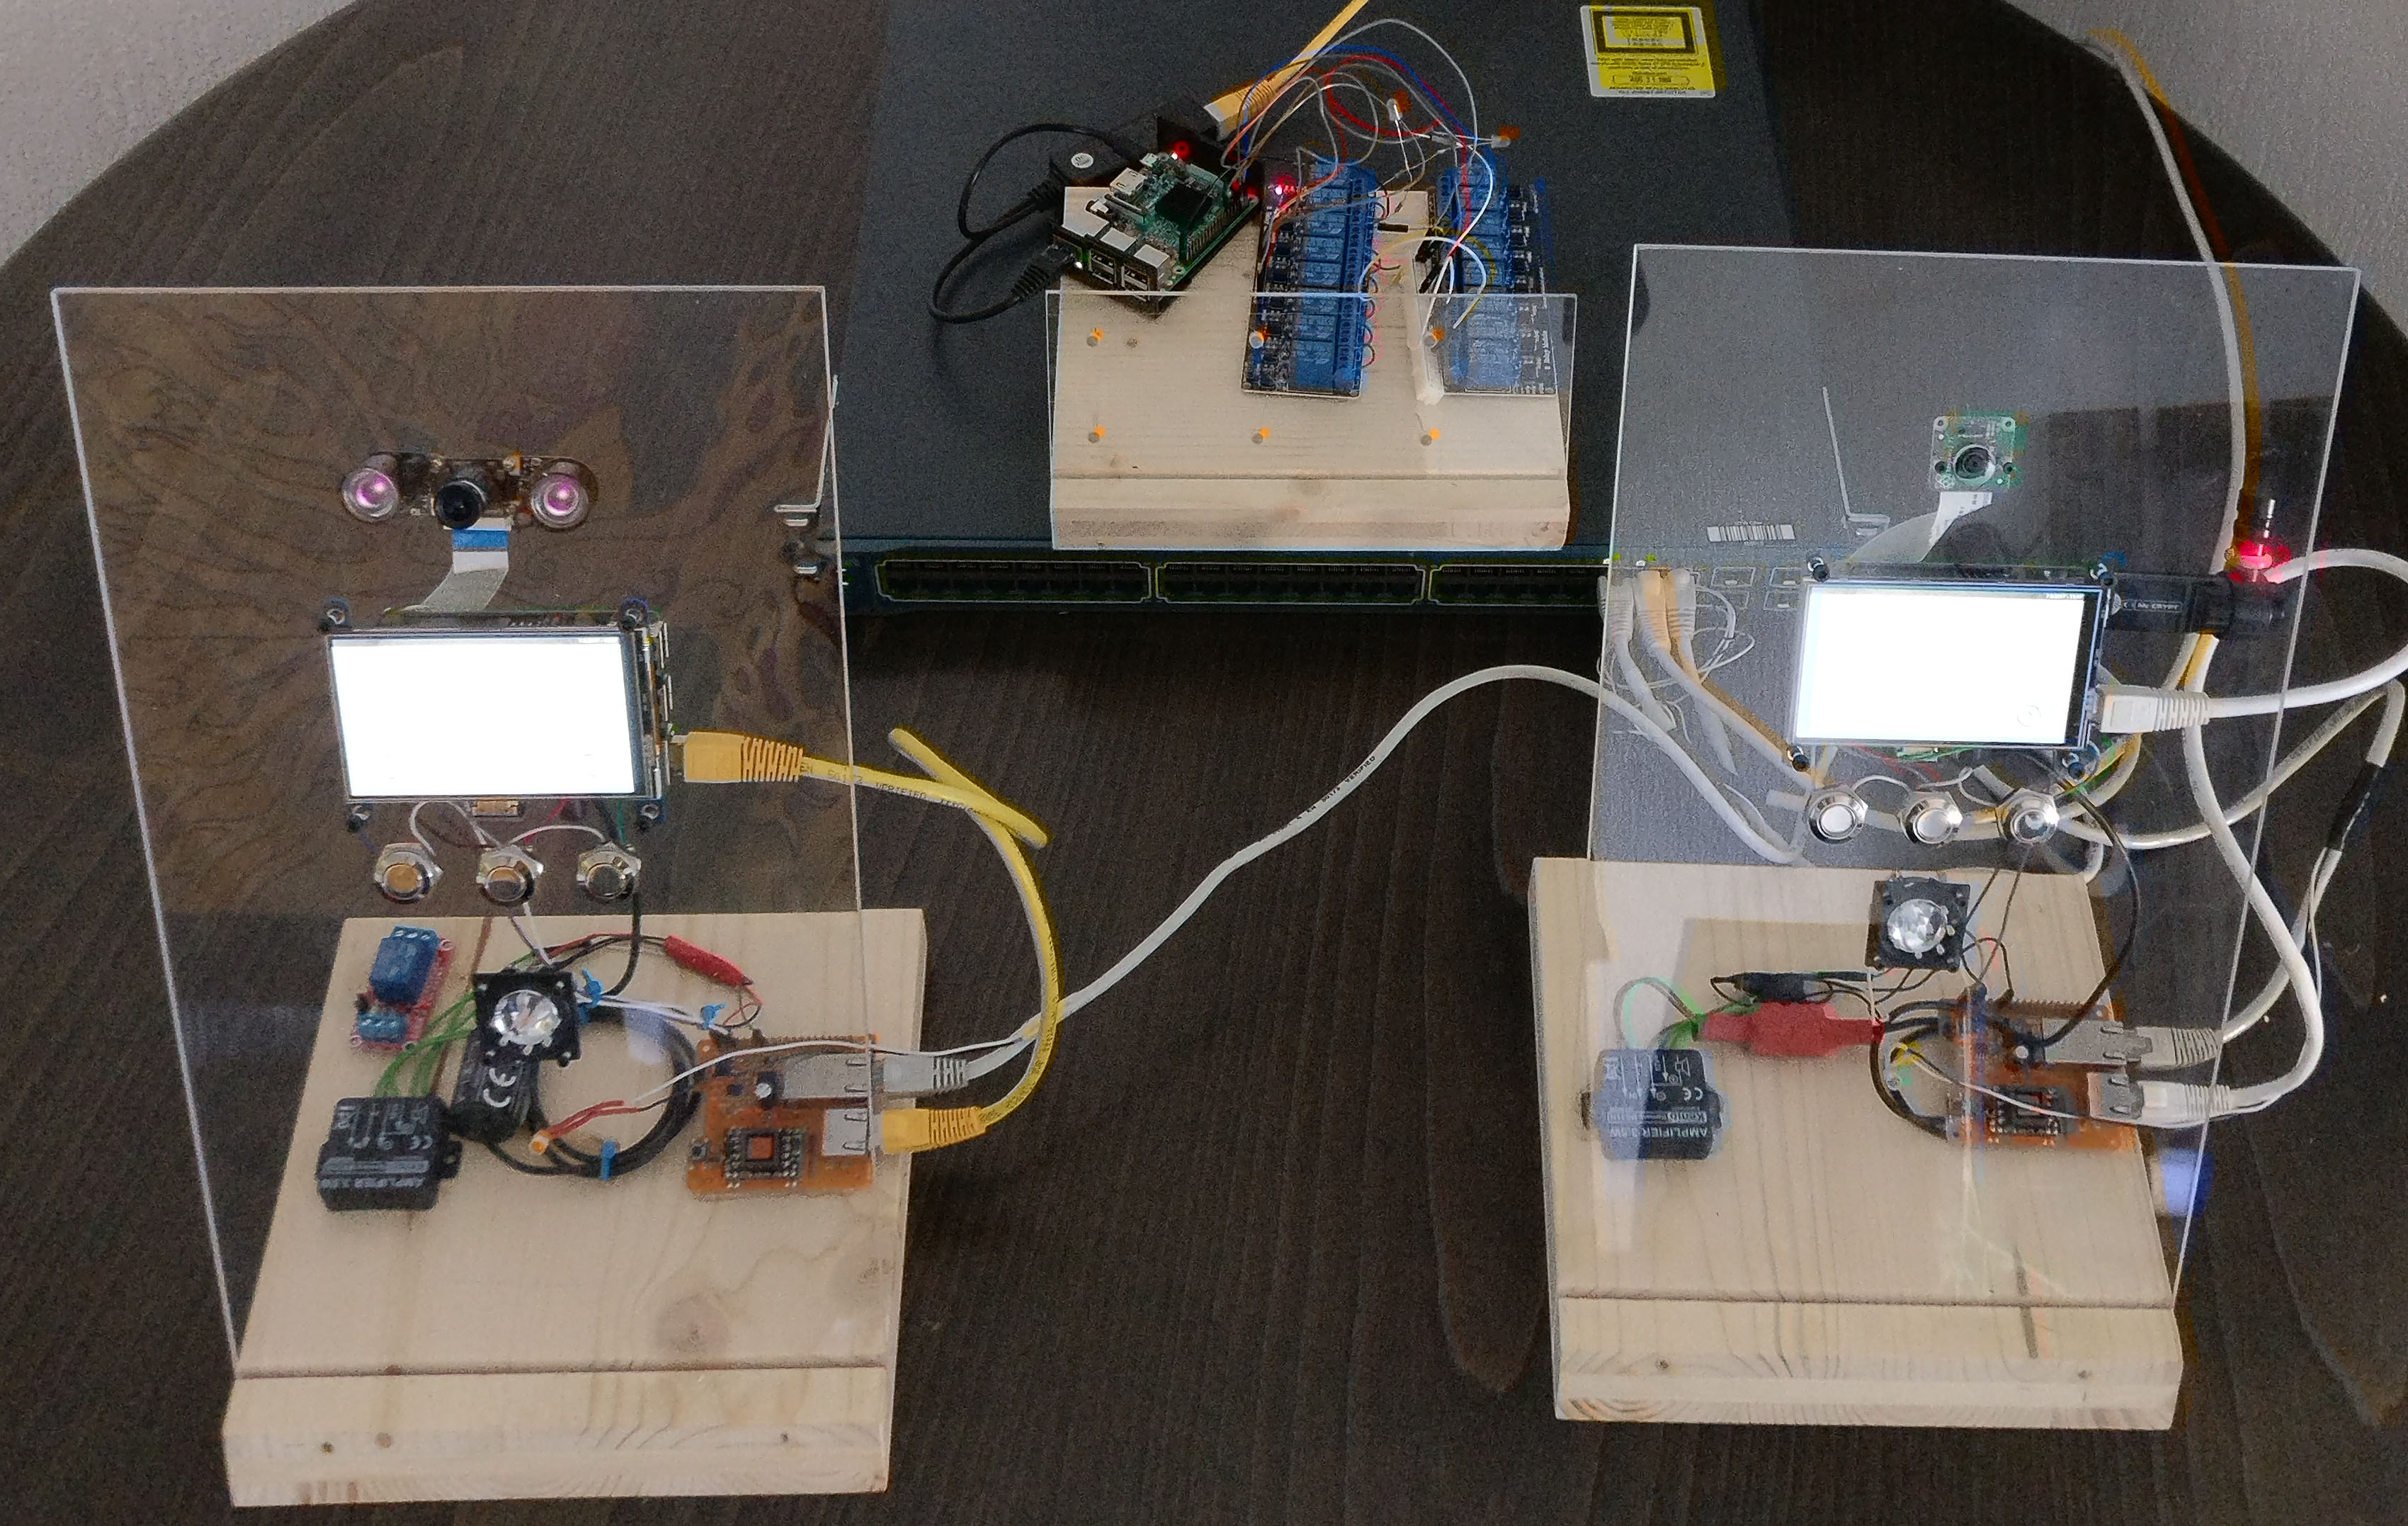
\includegraphics[width=0.95\textwidth]{prototyp}
		\caption[Prototyp Foto]{Präsentation Prototyp}
		\label{fig:prototyp}
	\end{center}
\end{figure}
\newpage







